\documentclass{beamer}
\usepackage{graphicx}
\usetheme{Manhattan}
\title{From Individual\\to Population\\\Large (Challenges in Medical Visualization)}
\author{Maarten Inja, Chiel Kooijman}

\begin{document}
\begin{frame}
	\maketitle
\end{frame}

\begin{frame}
	\frametitle{The 70s: 2D}
	\begin{itemize}
		\item CT \& MRI
	\end{itemize}
	\begin{center}
		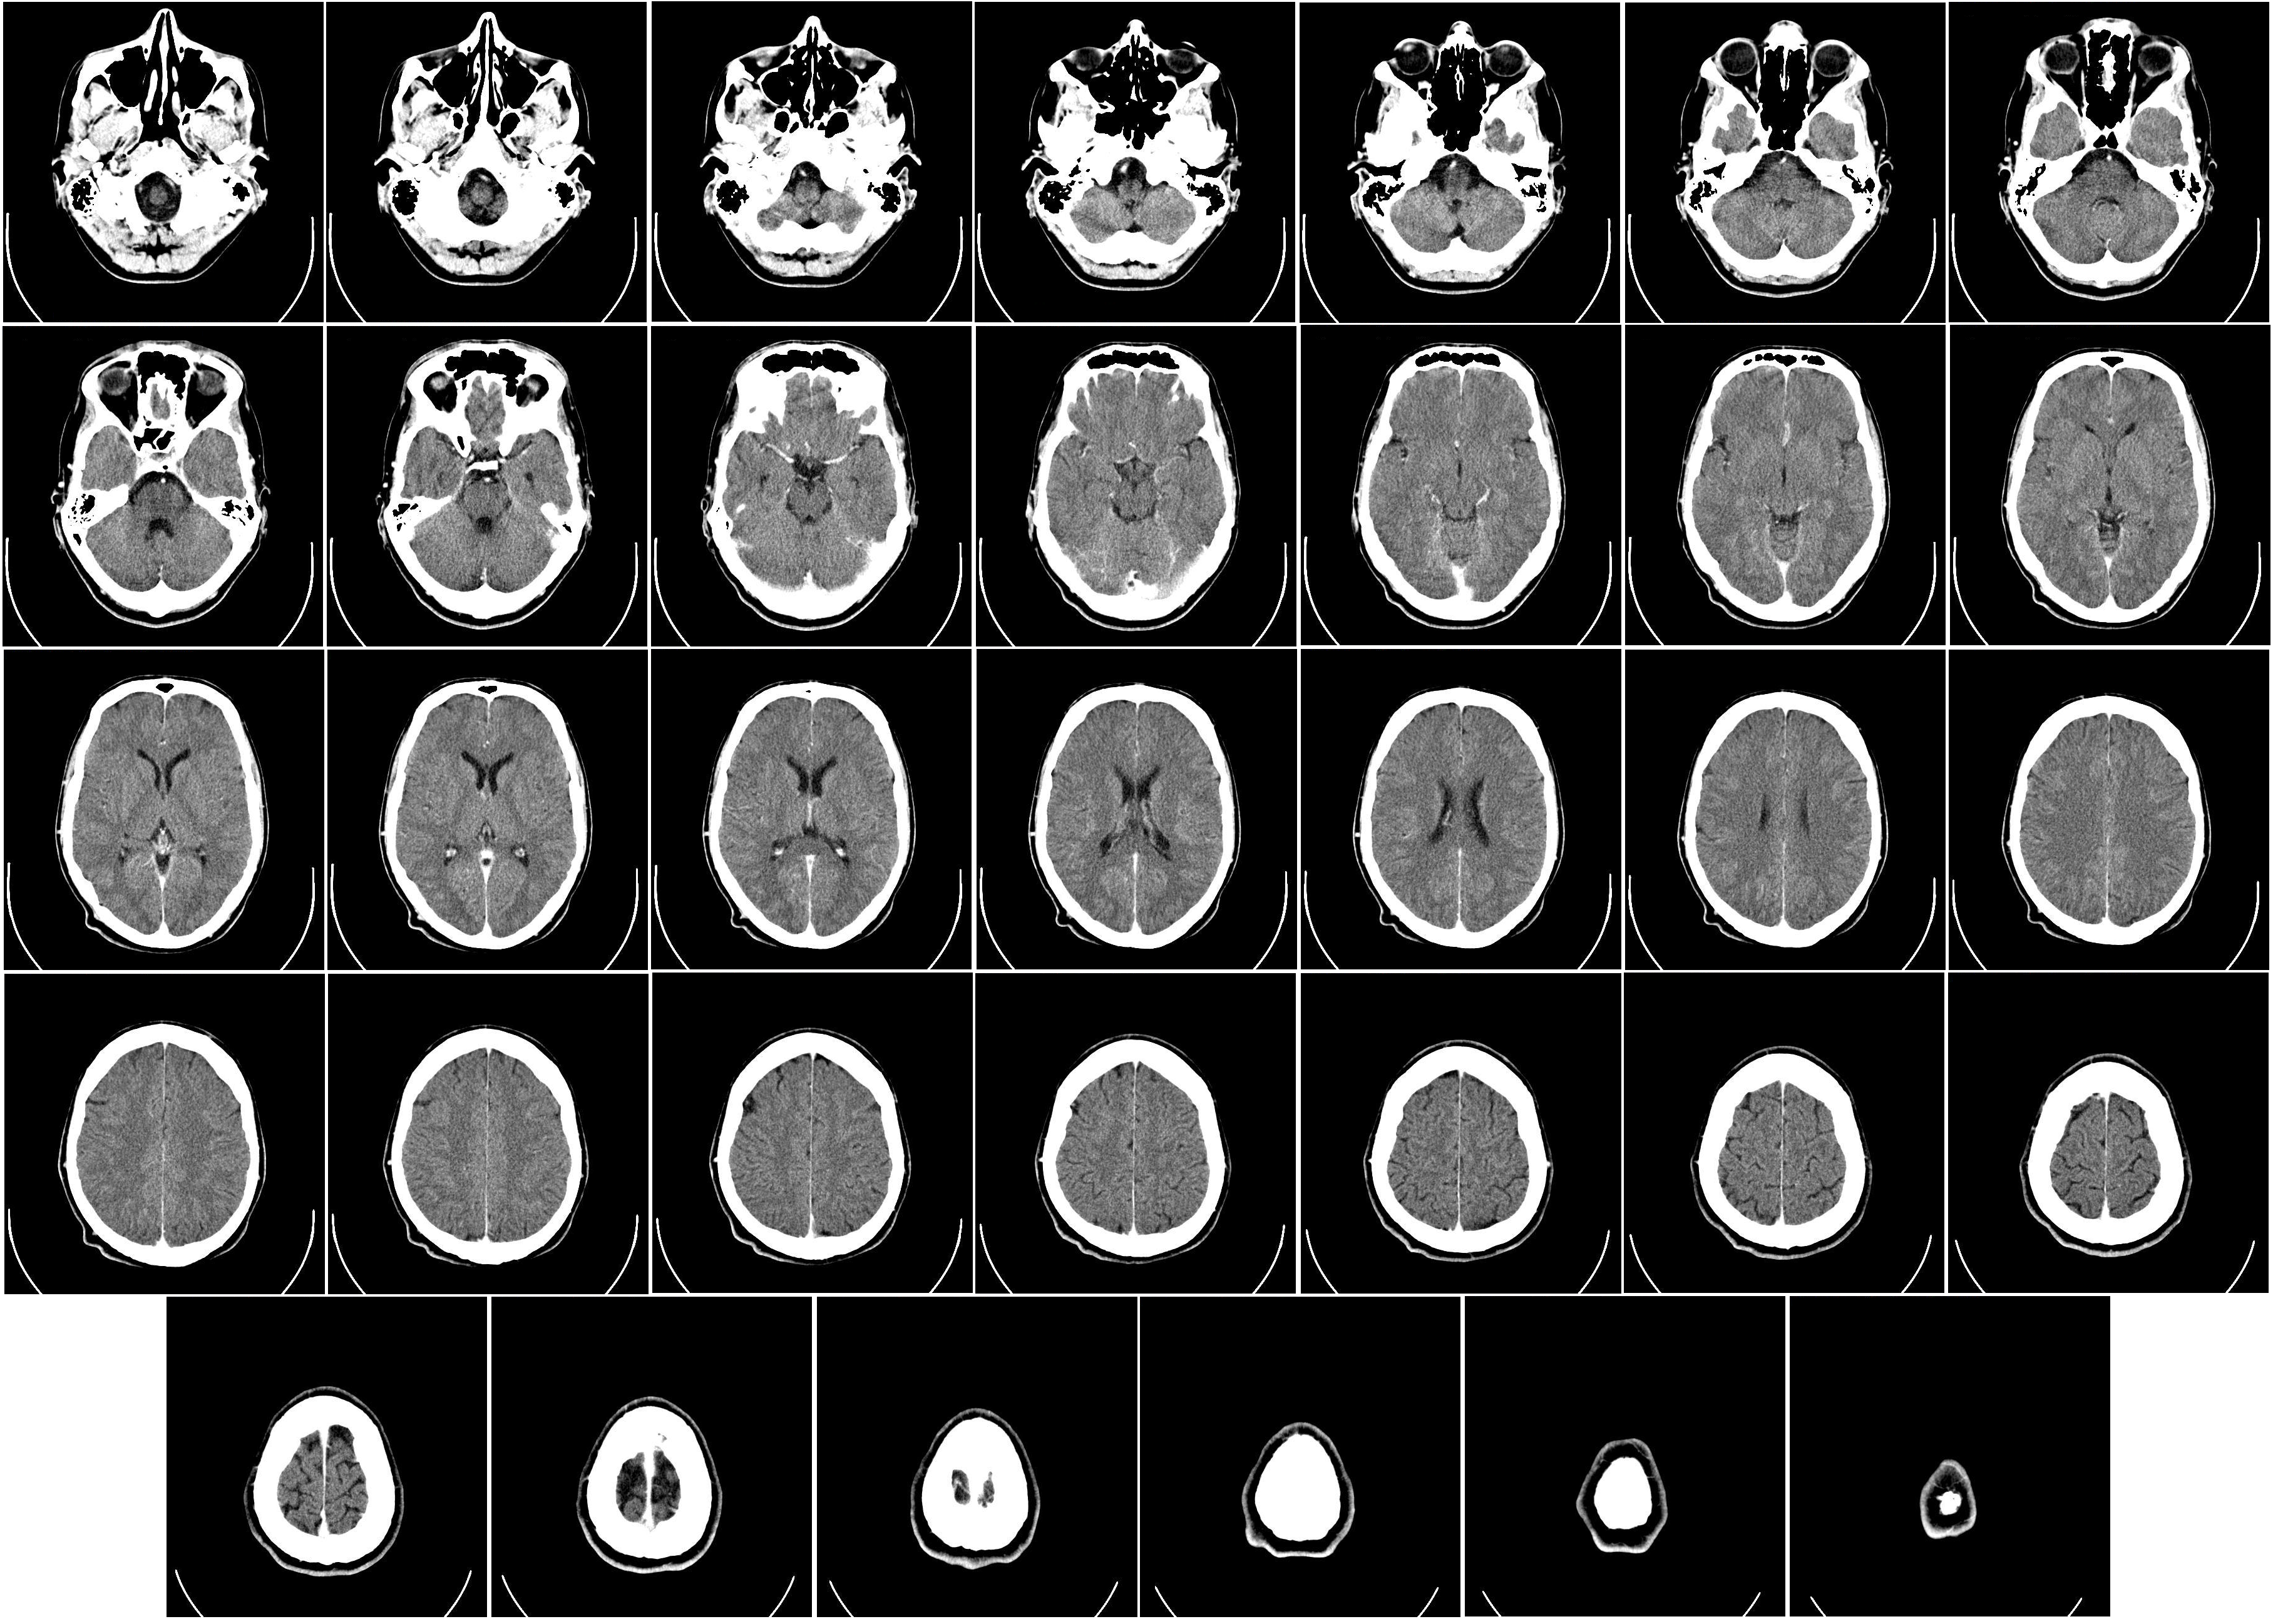
\includegraphics[width=.6\textwidth]{images/ct}
	\end{center}
\end{frame}

\begin{frame}
	\frametitle{1987: 3D}
	\begin{itemize}
		\item Marching Cubes/Isosurfaces (CT)
	\end{itemize}
	\begin{center}
		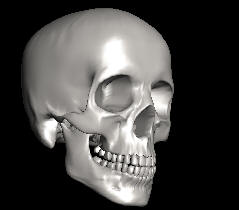
\includegraphics[width=.4\textwidth,height=.4\textheight]{images/marching}
	\end{center}
\end{frame}

\begin{frame}
	\frametitle{More dimensions}
	Higher dimensional data due to:
	\begin{itemize}
		\item Time-variance
		\item Multi-field (DTI, tensors)
		\item Simulation
		\item Multiple sources
			\begin{itemize}
				\item Multi-subject
				\item Multi-modal
			\end{itemize}
	\end{itemize}
\end{frame}

\begin{frame}
	\frametitle{More dimensions}
	\textbf{Solutions:}\\
	Add interactivity:
	\begin{itemize}
		\item Multi-touch devices allow for more flexibility
	\end{itemize}
	Improved visualizations:\\
	\begin{itemize}
		\item Topological methods
		\item Illustrative visualizations
	\end{itemize}
	versus
	\begin{itemize}
		\item Hyper-realism
	\end{itemize}
\end{frame}

\begin{frame}
	\frametitle{2001: 4D}
	\begin{itemize}
		\item Tory et al. (2001) use isosurfaces to visualise MS lesions over
			\textbf{time} (MRI)
	\end{itemize}
	\begin{center}
		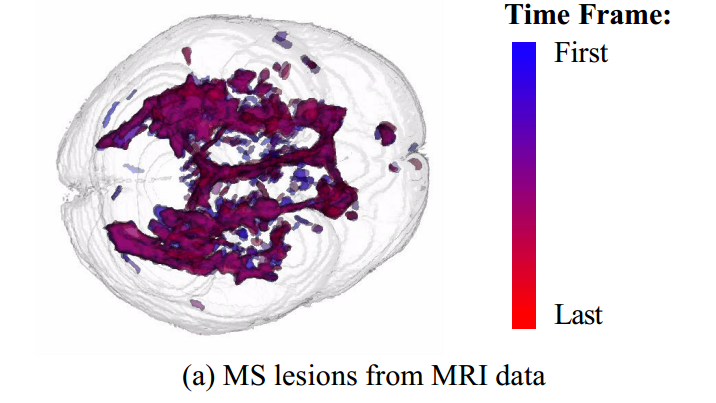
\includegraphics[width=.8\textwidth]{images/ms_time}
	\end{center}
\end{frame}

\begin{frame}
	Mappings:
	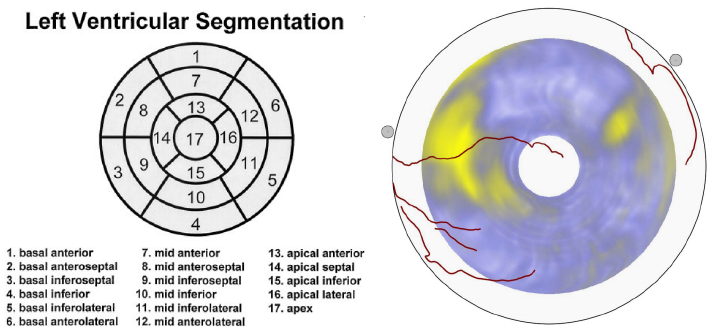
\includegraphics[width=\textwidth]{images/heart}
\end{frame}

\begin{frame}
	Illustrative (Zachow et al. 2009):
	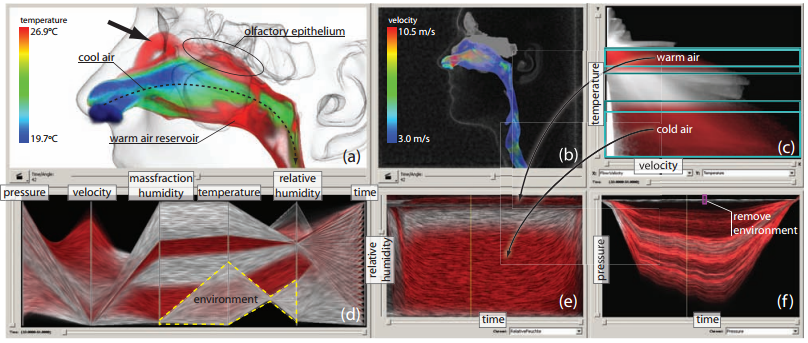
\includegraphics[width=\textwidth]{images/nose}
\end{frame}

\begin{frame}
	Illustrative - colon unfolding (Tietjen et al. 2005):
	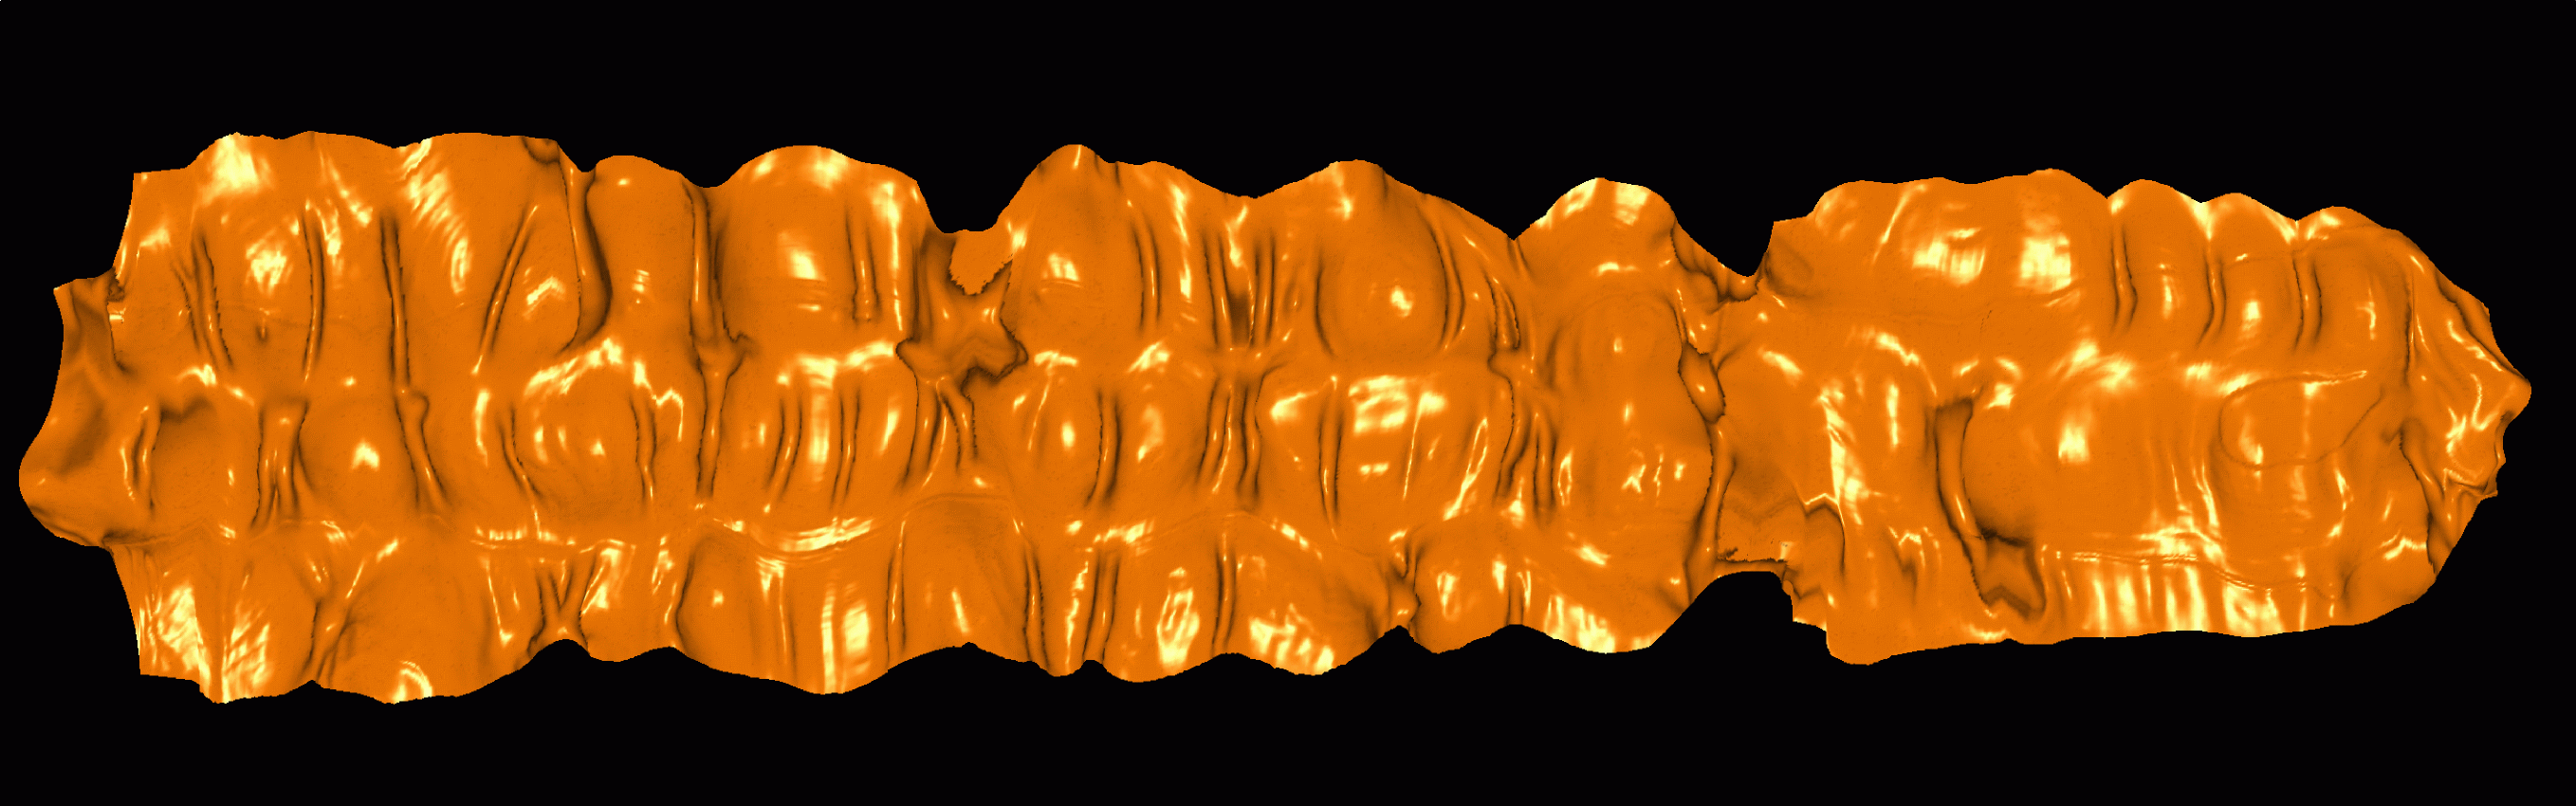
\includegraphics[width=\textwidth]{images/colon}
\end{frame}

\begin{frame}
	DTI (2.3):
	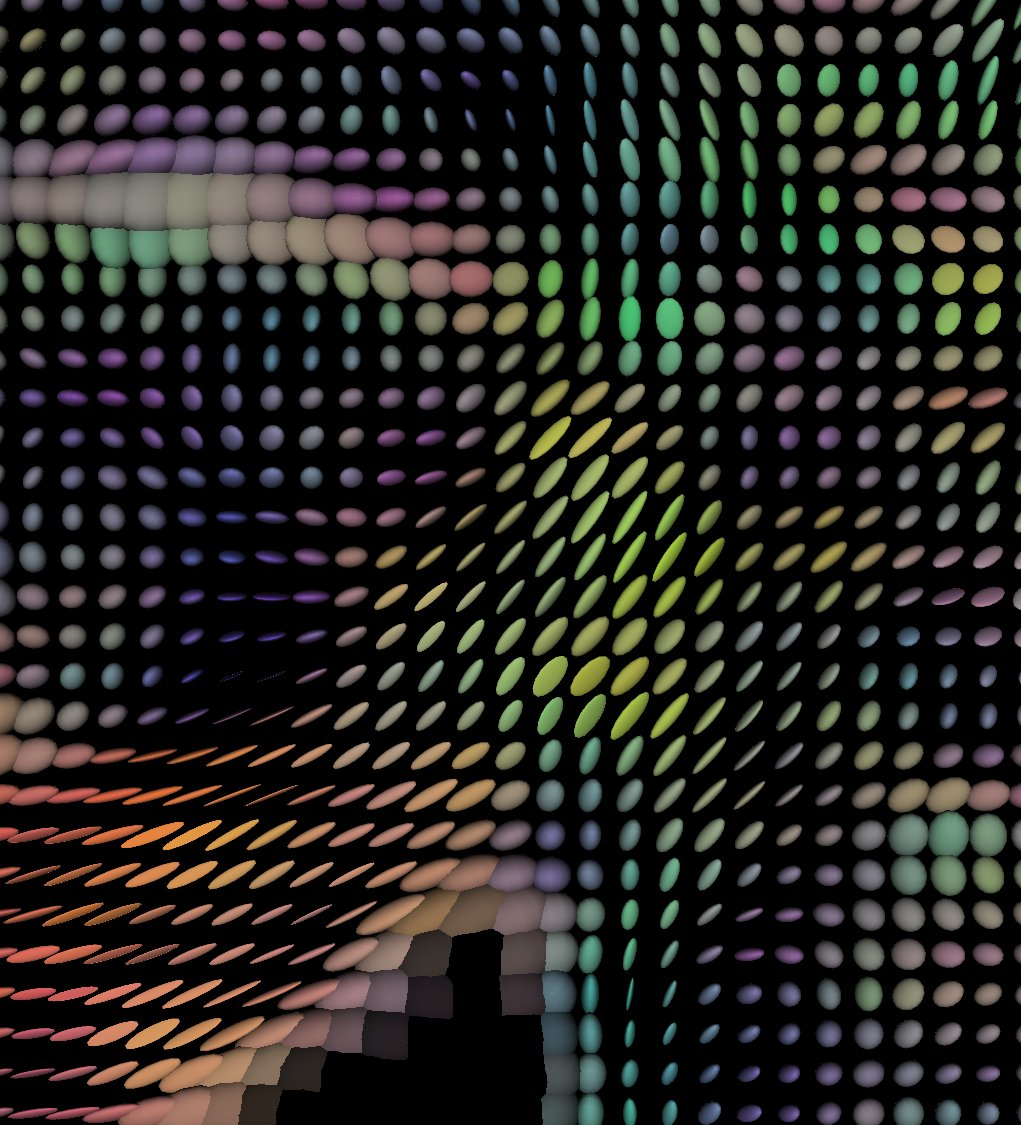
\includegraphics[width=\textwidth]{images/dti}
\end{frame}

\begin{frame}
	DTI (2.3):
	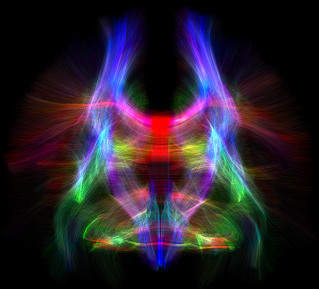
\includegraphics[width=\textwidth]{images/tractography}
\end{frame}

\begin{frame}
	Realism:
	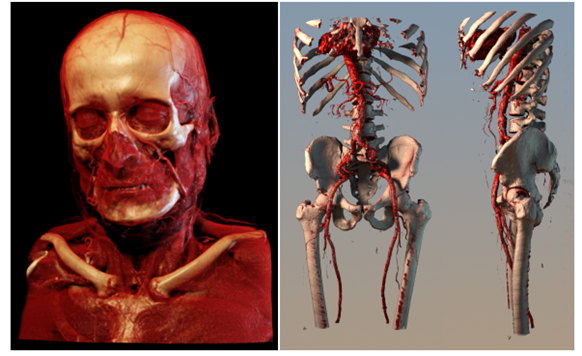
\includegraphics[width=\textwidth]{images/medical_visualisation}
\end{frame}

\begin{frame}
	Realism:
	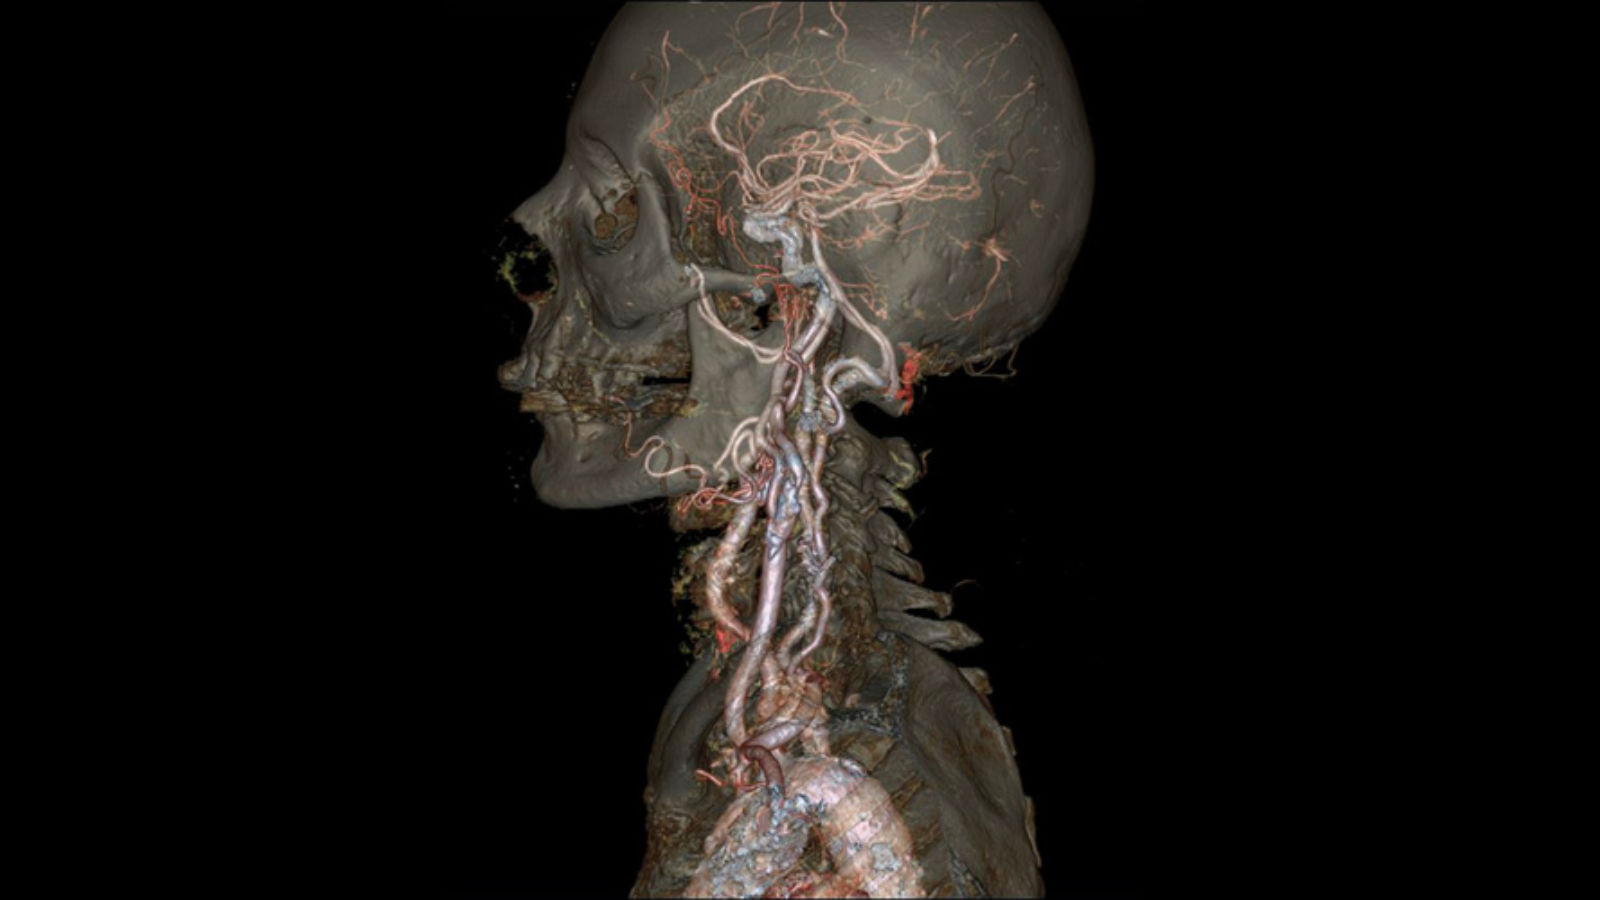
\includegraphics[width=\textwidth]{images/realistic_transparent}
\end{frame}
\end{document}
% vim: spell
